\documentclass{article}
\usepackage{graphicx}
\usepackage[a4paper, hmargin = 2cm, vmargin = 2cm]{geometry}
\usepackage[german]{babel}
\usepackage{wrapfig}

\title{Factsheet : Justiz}
\author{Oliver Baltisberger, Andreas Stoll, Melanie Rast, Christian Pernet}
\date{\today}

\begin{document}
	\maketitle
\subsection*{Das Problem der Gleichbehandlung}
«Gleiches gleich und Ungleiches ungleich behandeln», so lautet ein Grundsatz in der Rechtsprechung. Trotzdem kommt es manchmal zu «ungerechten» Urteilen, weil verschiedene Richter scheinbar gleiche Fälle unterschiedlich bewerten. Das Dilemma der Justiz besteht also darin, ein Gleichgewicht zwischen dem Gleichbehandlungsgebot und der individualisierter Rechtsprechung zu finden. Momentan wird dieses Dilemma i.d.R. mit gesetzlich vorgegebenen Mindest- und/oder Höchststrafen gelöst, innerhalb derer die Richter eine «angemessen» Strafe für den vorliegenden Fall festlegen können (z.B. wird Diebstahl in der Schweiz mit einer Geldstrafe oder einer Freiheitsstrafe von bis zu fünf Jahren bestraft). Jedoch gibt es eine bessere Lösung: Wenn nämlich ein Algorithmus Teil des Verfahrens ist, können sowohl Gleichbehandlung als auch individualisierte Rechtsprechung erreicht werden! 

\subsection*{Die Gerechtigkeitsgleichung} 

Algorithmen dürfen allein keine Schuld feststellen. Sie sind aber hilfreich, um die Wahrscheinlichkeit eines Rückfalls zu bestimmen. Sie werden seit den 1920er Jahren im Bereich der Justiz verwendet.  Ein solches Instrument wurde von dem Soziologe Burgess 1928 entwickelt. 21 Faktoren wurden berücksichtigt, u.a. bestrafte Tat, die Dauer der Haft oder auch der soziale Typ des Gefangenen. Jeder Faktor war 1 Punkt wert. Die Gesamtpunktzahl diente dazu, das Rückfallrisiko zu schätzen (Gesamtsumme hoch > Rückfallrisiko gering). Ergebnis: 98 Prozent der Personen mit niedrigem Risiko wurden während der Probezeit nicht rückfällig; bei 2/3 der Risikogruppe war dies der Fall. Diese Methode und die Faktoren wurden kritisiert (e.g. ist Kategorie “Bauernjunge” gültig?). Trotzdem wurde diese Methode in Illinois eingeführt und ihre Nachfahren weltweit eingesetzt. Die heutigen Algorithmen sind viel "raffinierter”. Das Prinzip bleibt jedoch dasselbe. Man gibt Fakten vor und eine Prognose wird geliefert, auf Basis einem Entscheidungsbaum. 

\subsection*{Der Publikumsjoker} 

\begin{wrapfigure}{r}{0.6\textwidth}
	\centering
		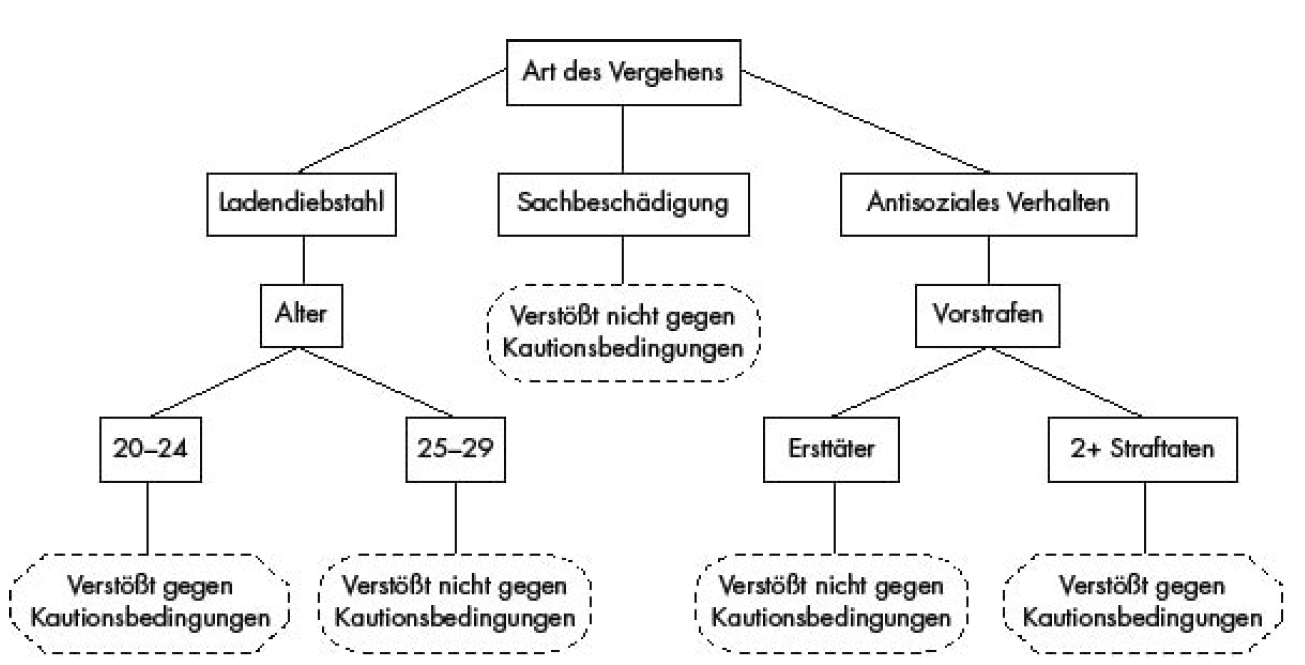
\includegraphics[width=0.58\textwidth]{D:/Christian/Desktop/divers/0phbern/justiz/tree.png}
		\caption{Einfacher Entscheidungsbaum}
\end{wrapfigure}


Ein Entscheidungsbaum kann angewendet werden, um festzustellen, ob ein Häftling gegen Kaution freigelassen werden kann. Mit Hilfe Daten früherer Häftlinge wird man Wahrscheinlichkeiten aufstellen können. Ein einfaches Beispiel dafür finden Sie in Abb.  1. 

Einen einzigen Baum zu bauen reicht leider nicht aus, auch wenn dieser mit einer sehr großen Datenmenge gefüttert wird. Wir werden sehr viele Entscheidungsbäume verwenden, die eine Menge bilden. Nicht alle Bäume werden die gleiche Antwort liefern. Der Durchschnitt wird jedoch relevant sein (Es funktioniert einigermassen wie der “Publikumsjoker” bei “Wer wird Millionär”).  

Diese Menge von Entscheidungsbäumen bilden einen Zufallswald, der als selbstlernender Algorithmus betrachtet wird. Diese werden z.B. von Netflix, Airbnb aber auch Gesundheitssystemen verwendet. Im Bereich der Justiz hat der Algorithmus jedoch den Vorteil, dass er immer die gleiche Entscheidung unter den gleichen Bedingungen trifft. Auch die Vorhersagen werden besser. 

\subsection*{Mensch versus Maschine} 

Im Jahr 2017 konnten Forscher mit Hilfe von Daten von New Yorker Straftätern aus den Jahren 2008 bis 2013 (insgesamt 0.75 Millionen) untersuchen, wie Algorithmen im Vergleich zu menschlichen Richtern urteilen. Im Nachhinein wurden die von Richtern beurteilten Fälle Algorithmen zur Beurteilung vorgelegt. Von den von den Richtern auf Kaution freigelassenen Straftätern erschien über die Hälfte nicht vor Gericht und noch mehr wurden wieder straftätig, vieles davon wäre von Algorithmen korrekt vorhergesehen worden. In Rhode Island, wo seit ein paar Jahren Gerichte Algorithmen für die Urteile verwenden, werden nun 17\% weniger Menschen ins Gefängnis gesteckt und 6\% weniger Straftäter rückfällig. 

\subsection*{Auf der Suche nach Darth Vader}

Bei einer Prognose bezüglich Kriminalität (bzw. allgemein) sind zwei Fehler möglich: 
 
		\begin{itemize}
			\item Falsch-negatives Ergebnis: Eine Person, die ein Risiko darstellt, 
						wird nicht erkannt. 		
			\item Falsch-positives Ergebnis: Eine Person wird zu Unrecht als 
						Risiko eingestuft. 
	\end{itemize}

Der momentan genauste Algorithmus im Justizbereich (Berks Algorithmus) kann Morde mit 75\% Genauigkeit vorhersagen. Dies führt dazu, dass einigen Personen zu Unrecht als Mörder eingestuft werden. 

Ein Problem ist, dass bei der Entscheidung über die Länge einer Strafe nicht nur das Risiko einer Rückfälligkeit beachtet werden muss. Es stellen sich auch Fragen der Rehabilitation oder der Vergeltung.  

Algorithmen können auch zu wenig intuitiven Urteilen führen. So bewertet der COMPAS-Algorithmus ein tiefes Alter eines Täters negativ, auch wenn bei einem Sexualstraftäter, welcher Geschlechtsverkehr mit einer Minderjährigen hatte, dies bedeutet, dass der Altersunterschied kleiner war. 

Es besteht auch die Befürchtung, dass sich Richter, welche in den USA gewählt werden, aus Angst vor Fehlern zu sehr auf Algorithmen abstützen. Wenn ein Algorithmus zu einem falsch-positives Ergebnis gelangt, kann dies nie mit Sicherheit festgestellt werden: Vielleicht wäre die Person ja wirklich straffällig geworden. 

\subsection*{Maschinelle Vorurteile} 

\begin{wrapfigure}{r}{0.6\textwidth}
	\centering
		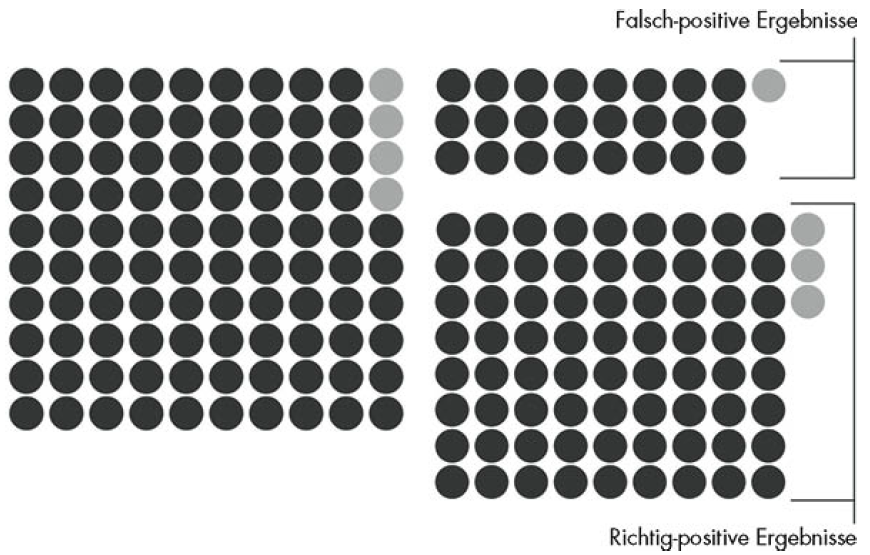
\includegraphics[width=0.58\textwidth]{D:/Christian/Desktop/divers/0phbern/justiz/results.png}
		\caption{Richtig- und Falsch-positive Ergebnisse}
\end{wrapfigure}

Die Hautfarbe wird vom Algorithmus COMPAS nicht explizit als Faktor einbezogen, aber die Art der Fehler unterscheidet sich. Unter den falsch-positiven Ergebnissen gab es unverhältnismässig viele Schwarze und bei den falsch-negativen Ergebnissen unverhältnismässig viele Weisse. Ein fairer Algorithmus sollte unabhängig von der Hautfarbe dieselben Einschätzungen machen und eine gleiche Fehlerquote aufweisen. Das Problem ist, dass dies mathematisch gar nicht möglich ist. Dies lässt sich anhand folgender Abbildung zeigen: 96\% aller Morde werden von Männern (dunkle Kreise) begangen und nur 4\% der Morde von Frauen (helle Kreise). Wenn nun der Algorithmus zu 75\%iger Wahrscheinlichkeit die Mörderquote korrekt voraussagt, werden rein aus mathematischen Gründen mehr unschuldige Männer als Frauen fälschlicherweise des Mordes bezichtigt. Solange die Bevölkerung bei Straftaten nicht anteilsmässig gleich vertreten ist, kann kein Test prozentual gleich viele Fehler machen.  

\subsection*{Schwierige Entscheidungen}

Es stellt sich die Frage, ob Algorithmen aus der Justiz verbannt werden sollen. Doch diverse Studien zeigen, dass Richter diskriminierende Urteile fällen, auch ohne explizite Vorurteile. Denn unser Denken fusst auf zwei Systemen: Das schnelle, automatische, intuitive und das langsame, überlegte, reflektierte. Wir Menschen können grosse, komplexe Probleme nicht rational und logisch erfassen, ohne dass das intuitive System mitspielt. Da auch Richter nur Menschen sind, spielt ihre Intuition eine grosse Rolle bei der Aufrechterhaltung der Verzerrungen im System.  

\newpage

\subsection*{Mögliche Fragen} 
		\begin{enumerate}
			\item Darf geistiges Eigentum (COMPAS) über Gerechtigkeit / Nachvollziehbarkeit stehen? 
			\item Können falsch-positive Vorhersagen von einem Menschen eher 
						akzeptiert werden als von einer Maschine? 
			\item Sollte in Algorithmen die aktuelle Wirklichkeit repräsentiert 
						werden (auch wenn diese ungerecht ist)? 
			\item Ist eine Diskriminierung von Maschinen schlimmer als eine von Menschen? 
			\item Sollte man den Richtern diesen Ermessenspielraum nehmen? 
\end{enumerate}
 
	
\end{document}